\documentclass{article}
\usepackage{textcomp,verbatim,amssymb,amsmath,array}
\usepackage{vo}
\pagestyle{empty}
\begin{document}


\title{VersoTeX, a LaTeX style for producing a dynamic HTML}

\author{Oleg Viro}
\date{}

\maketitle

VersoTeX prepares dynamical HTML documents for reading in a web-browser. 
A source file looks like a usual source LaTeX file. 

VersoTeX can be applied to a paper written in a plain LaTeX article style. 
If you write your papers in TeX, you can adjust any of them to VersoTeX. 
Although most of more sophisticated styles are not yet supported, virtually 
any LaTeX file after appropriate adjustments can be handled by VersoTeX.
Indeed, the last 15 articles published in the
\url{http://armj.math.stonybrook.edu}{Arnold Mathematical Journal}
have been transformed into a dynamical HTML format by VersoTeX, and 
most of articles published in the first two years in the
Arnold Mathematical Journal were transformed by a similar package.

VersoTeX has a number of features. They are described below. 
The main purpose of them is to make reading and a careful study
of text convenient. Dynamic HTML provides opportunities for this, 
which are not available for paper publishing or pdf.

When reading a mathematical text, we meet 
numerous references: to literature, to formulas, definitions and statements
of theorems from other parts of the text, etc. Often the reader wants 
to see some of them simultaneously with each other and the text 
which is currently read. On the other hand, at first reading we prefer  
to move out of the sight some details, like proofs. VersoTeX allows to 
do all of this. 

\section{Instructions to a VersoTeX reader}\label{s1}
\subsection{Three fields}\label{s1.1}
When you open in a web browser window (which is wide enough) 
an HTML document prepared as a TeX file 
with VersoTeX, you see a picture like this:\newline
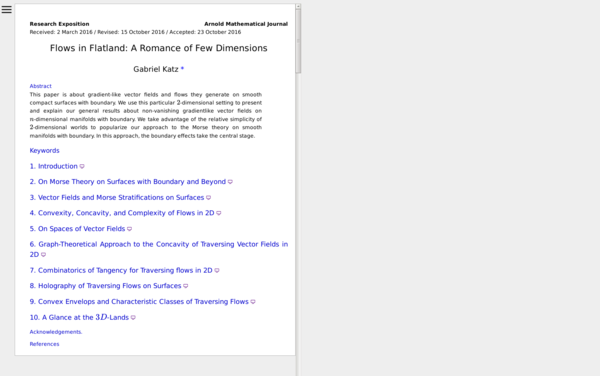
\includegraphics{figs/page-1.png} 

The page is divided into three fields. The leftmost one  
is narrow, just about 40 pixels wide, the middle one is of about 740
pixels. If the browser window is narrow, then the fields overlap.

On the top of the narrow field, there is an icon
\icon{icons/menu.png}. Usually such an icon hides a drop-down menu. Indeed, 
clicking the icon unrolls a menu.
We will describe its items later.
\lpict{
\includegraphics{figs/menu.png}}


\rpict{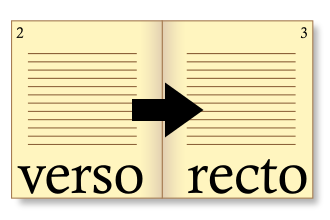
\includegraphics{figs/rectoAndVerso.png}}
The other two fields have names: the central one is called {\em verso\/}
and the rightmost is called {\em recto\/}. These are the names of left and
right pages in an open book. See
\url{\begin{onlyHTML}https://en.wikipedia.org/wiki/Recto_and_verso\end{onlyHTML}}{Wikipedia, Recto and
verso} 

When you open an HTML document, the recto field is empty. 

\subsection{Verso}\label{s1.2}
The verso field  looks like the beginning 
of a mathematical paper (including its abstract) followed by a 
table of contents. 
In fact, this is not a table of contents, but rather the whole
article folded down. Its blue lines are clickable. A click on the word 
``Abstract'' folds down the text of abstract leaving visible out of it 
only the word Abstract. 

The lines below the abstract are titles of sections. 
A click on each of them unrolls the section. 
If the section contains subsections, then each of the
subsections is still folded and is represented by its title. 
Clicking the title unfold their content. Clicking the title of an 
open fold folds it down.

This folding  format is broadly used in programmer editors and in online 
tables of content. It allows to keep out of sight parts of the text that 
are not of interest at the moment. 

It takes time to unfold a text section by section. An inpatient reader may 
open all the folds by at most two mouse clicks. Open the menu 
(this requires a click if the menu was not open) and click the icon 
\icon[height=19px]{icons/goBottom.png} 
The next icon \icon[height=19px]{icons/goTop.png}
 closes all the folds
(including the abstract) at a single click.

At the bottom of each open fold there is a thin (one pixel thick) blue line.
Under mouse it becomes thicker. When clicked, it folds down the fold above
it. So, if you have read a section (or a subsection) and want to close the
fold, you can use this line instead of clicking the title of the section
after going all the way up to it. 

In addition to sections, subsections and subsubsections, 
there are other parts of
the text which can be folded and which by default are folded when you open 
the document.
These are special sections, like {\em References, Acknowledgements, Keywords, 
Mathematics Subject Classification\/}, and, besides, folds of a 
different nature: proofs. 
Of course, proofs are very important, but at the first
reading we often do not want to go into details. 

The title of a proof is blue and clickable. The click unfolds the proof.
At the end of an unfolded proof, we see a square 
\<span class="qed"\>\&\#11036\</span\> symbolizing the end of 
the proof.
Clicking the square closes the text of the proof.
   
Literature references are also blue and clickable. A click at a reference 
raises a small window with the relevant bibliographical data. 
The next click at the
same reference deletes the window. 

The window is
draggable. Draggability is handy, because when you click several 
references that are close to each other on the page the windows may
overlap, and you have to separate them by dragging.

A similar mechanism is implemented for footnotes. Thus a footnote becomes
a flying note and flies quite close to the place where you
clicked to the reference (so, you do not need to look at the bottom of the 
page or even at the bottom of the next page).

\subsection{Recto}\label{s1.3}
At the opening of a document, the rightmost field of the browser page, the
{\em recto\/} is empty. It's your choice, what to bring there. After a
while, it may look like this.\newline
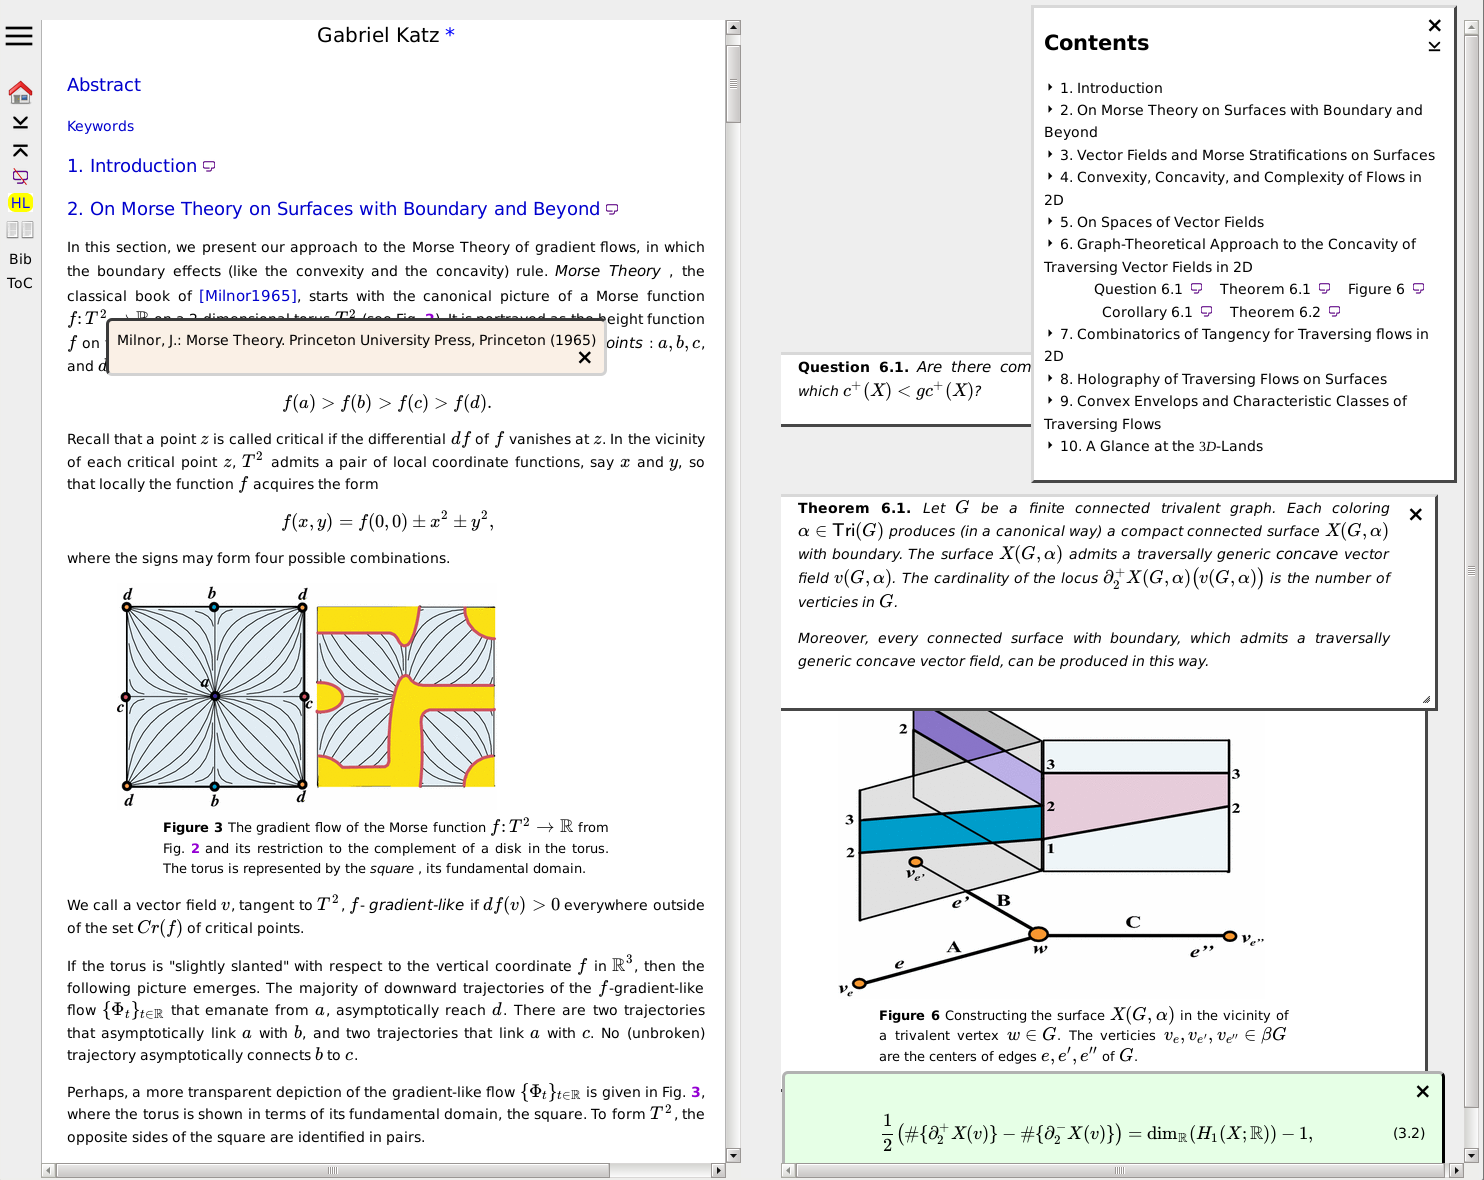
\includegraphics[width=600px]{figs/page-2.png}


\subsubsection{Table of Contents}\label{s1.3.1} 
A click on the bottom icon ToC in the menu brings up a Table of Contents
window at the right upper corner of the recto. The table of contents is 
folded and can be unfolded either gradually by clicking on triangles
\icon[height=12px]{icons/panStart.png} next to each item,  
or by a single click on the icon  \icon[height=15px]{icons/goBottom.png} 
on the right side of the table of contents window.

A click on an item of the table of contents effects the verso: it 
brings up the title of the corresponding part to the article. If the part 
was hidden in a closed fold, then the click opens all the folds that 
hide this part. 

Besides sections, subsections and subsubsections, the table of contents
lists also all the theorems, lemmas, corollaries, figures, tables, etc.


\subsubsection{From verso to recto}\label{s1.3.2} On verso, there are 
elements colored with dark violet. These are the numbers in references 
to sections, theorems, lemmas, and references to mathematical formulas. 
Clicking at any violet element creates on the recto a window
 with the copy of the corresponding part of the text. 
Those windows are draggable and resizable. A repeated click on the same
violet element of the verso closes the window on the recto.

On the verso, at the end of a title of a section/subsection/subsubsection, 
there is an icon  \icon[height=12px]{icons/bubble.png}. A click on that 
icon creates on the recto a window with a copy of the  
section/subsection/subsubsection. 

\subsection{Menu}\label{s1.4}
You can open a copy of the whole document on the recto, by clicking the
icon \icon{figs/double.png} in the menu. This gives a useful opportunity 
to reed side by side different parts of the document.

The icon Bib in the menu creates on the recto a window with a copy of the
whole bibliography.  

If you have got tired of these windows flying on recto or verso, you may 
kill all of them by a single click on the icon 
\icon[width=15px]{icons/crossedBubble.png} in the menu. 
Killing of a single window can be done also by
clicking a cross icon  on its upper right corner.

The menu icon \icon[height=15]{icons/HL.png} highlights all the 
pieces emphasized in the source tex file by the command
\begin{verbatim}\em\end{verbatim}.


\subsection{The environment for reading VersoTeX html article}\label{s1.5}
Of course, a modern web-browser is needed. This may be Firefox or any 
other clone of Mozilla, Chrome, Safari, Opera, Microsoft Edge, or even 
Internet Explorer.

The VersoTeX relies on MathJax, an open source display engine for
mathematical formulas. MathJax can work from a distributed network service, 
but, in order to use it in this way, one needs a web access. Also, one can
install MathJax in a local computer. See 
\url{https://www.mathjax.org/}{www.mathjax.org}

To a much lesser extent, VersoTeX uses jquery javascript library. They
also can work directly from the web, or can be downloaded to computer 
and work locally. See \url{https://jquery.com/}{jquery.com} and 
\url{https://jqueryui.com/}{jqueryui.com} .

In the setup provided here, we assume using content delivery networks.
In this version, displaying html files compiled by 
VersoTeX requires a web access.  
Besides, the following files are required:  
\begin{itemize} 
\item {\em vo.js}, a collection of javascript marcos;
\item {\em vo.css}, a Cascading Style Sheets for displaying html files produced
by VersoTex;
\item a directory {\em icons} with a few icons. 
\end{itemize}

They can be placed differently, but, in the configuration provided here, they
are placed in the same directory as the html file and, if one wants to have
them somewhere else, then a minor change of configuration would be needed.


\section{Instructions to a VersoTeX runner}\label{s2}
This section is addressed to a person who wants to run VersoTeX.
First, it was called {\em Instructions to an author}. But besides
authors, other people also can find it useful. 
If you have downloaded a paper from ArXiv with a serious 
intention to study it carefully, you may also want to improve 
its readability by VersoTeX.   

\subsection{Adjust the source file}\label{s2.1}
For the best result, the document class of the paper should be
article. So the source file should start with\newline
\<code\>
\begin{verbatim}
\documentclass{article}
\end{verbatim}
\newline
\begin{verbatim} 
\usepackage{verbatim,amssymb,amsmath,array}
\end{verbatim}
\newline
\begin{verbatim} 
\usepackage{vo}
\end{verbatim}
\newline
\begin{verbatim} 
\pagestyle{empty}
\end{verbatim}
\</code\>
Right after that you may put 
\<code\>
\begin{verbatim} 
\begin{document}
\end{verbatim}
\</code\>

Then it's a good place to introduce your customer commands for mathematical
formulas. Something like that:\newline
\<code\>
\begin{verbatim} 
\hide{$\newcommand{\Q}{\mathbb Q}$} 
\end{verbatim}
\newline
\begin{verbatim} 
\hide{$\newcommand\p{\partial}$} 
\end{verbatim}
\</code\>

Contrary to the usual practice, these definitions must be surrounded
with the dollar signs. The command \newline
\<code\>
\begin{verbatim} 
\hide{}
\end{verbatim}
\</code\>
\newline
is not necessary, but recommended. If you do not put it, the definitions
will be seen while the MathJax will be loading.

Then it's a right place to define your Theorem environments.
The amsthm.sty is not yet supported. Instead, the original LaTeX
commands can be used. Something like that:\newline
\<code\>
\begin{verbatim} 
\spnewtheorem{Th}{Theorem}[section]{\bf}{\it}
\end{verbatim}
\newline
\begin{verbatim} 
\renewcommand{\theTh}{\thesection.\Alph{Th}}
\end{verbatim}
\newline
\begin{verbatim} 
\spnewtheorem{rem}[Th]{Remark}{\bf}{\rm}
\end{verbatim} 
\</code\>

The environment proof is taken care of by VersoTeX, 
hence you do not need to define them here.

Abstract is a command rather than environment:\newline
\<code\>
\begin{verbatim} 
\abstract{The text of the abstract.}
\end{verbatim} 
\</code\>

The syntax for the commands 
\<code\>
\begin{verbatim}
\title, \author, \date, \maketitle, \section, \subsection, \subsubsection,
\label, \ref, \cite, \footnote 
\end{verbatim}
\</code\>
is usual. Inside math formulas everything is usual, or, to be more 
precise, as MathJax requires.

VersoTeX is good for handling files that are not too long. 
 I plan to work out a book version of
VersoTeX, in which this restriction will be lifted.
If a paper version of the file is about 50 pages or longer, 
then it's better to split it prior to feeding to the present VersoTeX.   
This restriction comes from MathJax. For a long files it takes too 
long to load MathJax. 



Answers to other TeX questions can be found in a few sample files
of articles by the author which you can find in this directory.   

Enjoy!

\subsection{The environment needed for running VersoTeX}\label{s2.2}
First of all, the TeX should be installed and working. Any major TeX
distribution, like TeX Live, Mac TeX or MikTex, should work. 

A TeX distribution usually contains a little program {\em catdvi\/}.
If this is not the case, install it separately: it is needed.

The process of compilation is organized by macros written in the Vim macro
language. Let me remind that Vim is a programmer's text editor, a 
clone of Vi. Vim is freely available for any operating system, see
\url{http://www.vim.org}{www.vim.org}.

Compiling a VersoTeX article requires an installed  VIM editor 
and two files: 
\begin{itemize} 
\item {\em vo.vim}, a collection of macros in the VIM macro language;
\item {\em vo.sty}, a LaTeX style file.
\end{itemize}

\subsection{Running VersoTeX}\label{s2.3}
Compilation of a LaTeX source file is performed as follows. 
The source file, say article.tex, is open in Vim. Then, the macros
from vo.vim are to be run in Vim. You just need to type in the command mode\newline
:source vo.vim\newline
Here we assume that vo.vim is located in the same directory as the source
TeX file.
Then vo.vim organizes the whole compilation. We consider the process of
compilation in the next section. In a regular situation, the process of
compilation does not require any user's action, except for pressing 
bar, when Vim says ``more'', and enter, when Vim requires.  

Vim shows red complain lines, when it fails
to find a regular expression, which had to be replaced. The user should not
care about these warnings. 
At the end of the process,
we find Vim open with the resulting file article.html open and this file 
saved in the directory, where article.tex was taken from.
 
\section{Under the hood}\label{s3}
Technically, VersoTeX is a LaTeX style supplemented with a few 
macros in the Vim macro language. 
This choice of tools was determined by the experience and expertise of the
author, who is not a programmer, but a mathematician. 
Perhaps, a programmer would use, instead of Vim, a more conventional 
engine, like PERL. As for the use of TeX engine, it has definite advantages. 
We will discuss them later.

As was mentioned above, a VersoTeX compilation of a TeX source file, say 
article.tex, starts with opening article.tex in Vim and typing\newline   
:source vo.vim.
The macros collected in vo.vim then do the following:
\begin{enumerate} 
\item Remove the files built by the preceding runs of vo.vim (if any).
\item Remove or replace a few TeX commands.
\item Localize mathematical formulas in article.tex, surround them with
a special markers, numerate formulas and insert in the beginning of 
each of them a special code containing the number of the formula.
\item Save the result as two files, M1-article.tex and T-article.tex,
identical to each other.
\item Open file M1-article.tex and erase in it everything besides the
formulas' codes and the formulas.
\item Each line in M1-article.tex is converted to a Vim macro which 
would replace the formula's code by the formula. After that the
file consisting of these Vim macros is saved as M1-article.vim.
\item In M1-article.tex, all lines, which contain no label, are erased, 
each line with a label turned into a Vim macro for placing two copies 
of the label around the formula code. The result is saved as M1-article.tex.
\item In T-article.tex the mathematical formulas are erased. Only the
formula's code is left in the place of each of the formulas. The codes of
formulas that were labeled are equipped with the copies of labels (using
the macros prepared in M1-article.tex),
\item In T-article.tex, around each environment with a label, vo.vim creates 
a germ of div container whose id is the environment's label.
\item In T-article.tex, the tabular environment is enhanced by inserting 
the commands which will force TeX to insert into each cell the information 
about its HTML class.
\item In T-article.tex the list of bibliography is duplicated and the TeX
commands in one of the lists are modified.
\item Some of the low level TeX commands are replaced. In particular, the
font type commands (like \begin{verbatim}\bf and \it\end{verbatim} 
) are 
replaced with commands, whose arguments are surrounded with braces (like 
\begin{verbatim} \textbf and \textit \end{verbatim}
).
\item Then vo.vim three times executes latex on T-article.tex.
\item vo.vim executes the command catdvi on T-article.dvi and 
saves the result as article.html.
\item In article.html, vo.vim makes the last cosmetic changes: 
unites the pages, removes unneeded brackets in references, insert the
horizontal lines into tables.
\item Finally, vo.vim inserts mathematical formulas into article.html 
by running M1-article.vim on it.  
\end{enumerate}

After this, the result is saved as article.html and stays open in Vim.
A number auxiliary files are left: M1-article.tex, M1-article.vim,
T-article.tex, T-article.toc, T-article.toc and T-article.log. They may be
useful only for debugging. 

Most of the job is done by TeX. The style file vo.sty redefines many 
usual LaTeX commands, so that they force TeX to draw, instead of usual 
typographical pages, an HTML file based on the same source file. 
   
\section{Speculations on problems and solutions}\label{s4}

\subsection{Two problems to be addressed}\label{s4.1}
TeX/LaTeX is a lingua franca of the scientific world.
Most of mathematicians and physicists write their research papers and
textbooks (and even private letters) in TeX/LaTeX. 
Most papers on ArXiv are prepared in TeX. (Lack of a 
TeX source for a paper in ArXiv is a strong indication that the author 
is not a professional.)

TeX and LaTeX are convenient for authors. Indeed, even if, when writing an
email, we need to include a mathematical formula, we use TeX codes, 
although it is not assumed to be processed by TeX. 

Now many documents are prepared for reading online from a computer screen.  
The screens become more readable. New generations of readers are used 
to read from screen. 

Still, one can use typesetting by TeX/LaTeX, convert the output to pdf format
and use Adobe Acrobat or other pdf-viewer. Although the picture that
appears on a computer screen is almost identical to the picture printed on 
paper, in some ways it is more convenient. It allows hyper-references and 
fast search of words.

However the pdf format does not allow to use many other new opportunities 
of the new media. It lacks most interactive capabilities of a 
simple web browser. 

The readers get used to appreciate advantages of interactive
texts. It seems that inevitably mathematics will find a way to publishing
online dynamic interactive texts.

There are two major problems to be solved for this:
\begin{itemize}
\item a convenient and useful design which would match the needs of a 
reader should be developed;
\item writer-friendly tools for preparation dynamic online documents
are to be developed.
\end{itemize}

\subsection{Design}\label{s4.2}
Hundreds of years of publishing worked out standards of a design 
for scientific papers. Just to make clear what I mean, let me mention 
a few elements of the design. Normally a paper has to be sectioned, 
although the number of levels in the sectioning may vary. 
Sections are equipped with titles. The list of bibliography is placed 
at the end of a paper.
The words defined in a definition is emphasized (e.g, by italic).
Statements of theorems are also distinguished with a font, equipped with 
titles and numbered. And so on...

For online dynamic publishing of scientific texts, the design principles 
and specific tricks are still to be developed. Usually the traditions of 
paper publishing are respected and followed, but enhanced occasionally 
with new elements. 
For example, a table of contents is made easily available (either it is 
permanently shown, or there is a button for displaying it) and the items 
of the table work as hyper-references.

I am not going to present a survey of works in this  direction, but
restrict to a few references to those works which were the most 
inspiring for me. 
\begin{itemize} 
\item\url{https://mathbook.pugetsound.edu/}{MathBook} by Robert A. Beezer is a
serious project in this direction.
\item 
\url{http://www.ams.org/publications/journals/journalsframework/AMSMathViewer}{AMS
MathViewer}
\item
\url{http://dlmf.nist.gov/LaTeXML/}{LaTeXML} by Bruce R.Miller\\ 
and the primary instigator for this project, the Digital Library of Mathematical Functions  
http://dlmf.nist.gov/
\end{itemize}

I use and agree with some design solutions coined in these projects, and
disagree with others. Below I formulate a few of design principles 
which I came to in my own project, VersoTeX.

\<p\>{\bf Dynamic design.} The same mathematical text is read with different
purposes (even by the same reader). For example, when you see a text for 
the first time, you do not want to see details of proofs, on the other
hand, you want to have
an easy access to definition, major statements and the list of literature. 
A design
should provide an opportunity to remove elements of the text off your sight 
at your wish, and emphasize other elements. This opportunity should be
self-evident. A reader should not be overloaded and confused by it.

\<p\>{\bf Folding.} There is an old simple way of dynamical hiding parts of
texts. It is implemented long ago in some programmer's text editors as
folding, see
\url{https://en.wikipedia.org/wiki/Code\_folding}{Wikipedia, Code Folding}  
It allows to hide the body of an element (e.g., a section, a proof), 
which can be made visible by a click to its title. It makes sense to
arrange the initial state of document such that only the title, authors,
abstract and a list of section headings is seen.

\<p\>{\bf The line lengths:}\newline 
{\bf Keep lines sufficiently short\/}, so
that it would not be difficult, after coming to the end of a line, to find
the beginning of the next line. On the other hand,\newline
{\bf keep lines sufficiently long\/} so that they accommodate  
mathematical formulas, which tend be long in some texts. 

\<p\>{\bf Justify text fully.} The text should be aligned along both margins.
This is a good option as long as lines are not too short.

\<p\>{\bf Inner references.} All references to other elements of the
text (bibliographic references, references to formulas, footnotes, theorems,
definitions, remarks, etc.) should be available without scrolling of the main 
text and realized by floating windows. These windows should be easy to open
and close. They should not stay on your way. Ideally, if the total width of
the browser allows, they should be placed in a separate area free of the main
text.  

\subsection{LaTeX for HTML}\label{s4.3}
The tools for preparation of dynamic online documents are not
writer-friendly. The very notion of a writer-friendly tool is to be 
specified. Here I mean a writer who knows LaTeX and has an experience in
writing source LaTeX files. Journal publications require this anyway.

The best solution for such a writer would be to write
a text file in an old good LaTeX, adding, when necessary, a few new 
commands for 
specific elements of the text. In other words, it is desirable 
to have a LaTeX style for preparing dynamic onscreen documents. The
closer this style would be to other commonly used styles for paper
publication, the easier would be to move between on-screen and on-paper
publishing of the same document.

A LaTeX source code contains almost all the information necessary
for creating dynamic HTML document fulfilling the design principles 
formulated above. It is divided into sections, subsections, etc.; 
statements of theorems, proofs, and definitions are distinguished; 
there is a built in system of internal and external references, etc.
Besides, it is easy to add new functionality via adding new commands
and environments. 

The tools available now require either learning the XML language or use of 
converter programs like LaTeXML.

A number of converters from LaTeX to dynamic html have been
written. The first of them, a PERL program LaTeX2HTML appeared in the
middle of nineties. 

Most of the existing LaTeX-HTML converters produce more or less literal
HTML copies of the paper. They are configurable, but changes are not
easy due to poor documentation. The most profound difficulty, which all 
converters faced, is a huge amount of style packages providing 
modifications and additions in TeX. 

The most convenient converter that I could
find so far is LaTeXML. I used it for making online version of the first
two volumes of \url{http://armj.math.stonybrook.edu/contents.html}{Arnold
Mathematical Journal.}
The necessary adjustments were made by Vim macros applied first to the source
TeX files and then to the resulting HTML files. Differences in
the author styles forced to make individual changes to almost each article.

VersoTeX is positioned as a style for LaTeX rather than a TeX-to-HTML
converter. It does not pursue the goal of automatic converting {\em any\/} 
TeX file to a valid HTML file. As other TeX styles, it is not a priori 
compatible with all other styles. 

Use the TeX itself as a parser and compiler is my original idea. It came
from experience. Like most mathematicians, I wrote mathematics in TeX.  
I did this for about 30 years, and besides, in the beginning of this 
period, I happened to write style TeX files for publishing of Russian journal 
\url{http://www.pdmi.ras.ru/AA/}{Algebra and Analysis}, and later I wrote 
style files for a textbook 
\url{http://bookstore.ams.org/mbk-54}{\textit{ Elementary Topology: Problem
Textbook\/}} and its Russian version. This experience convinced me that 
TeX is an adequate tool for drawing an HTML file as a picture based on a
TeX file. 

\acknowledgements{I am grateful to many people who helped. My daughter
Polina Viro wrote the first javascripts for VersoTeX and successfully hunted
numerous javascript bugs through the whole period of work. 
Raluca Tanase implemented canvas with justification of 
text and helped to maintain the web page of Arnold Mathematical Journal. 
At the first stage, I used LaTeXML developed by Bruce R.Miller. In
the HTML design I use many design solution from his work. I am grateful for 
very inspiring and fruitful conversations with Robert A. Beezer, 
David W.Farmer, Peter Krautzberger and Alexander Shumakovitch.}

\end{document}

There is a large community of TeX users. It includes virtually all
mathematicians and physicists. There is no reason to change the
input language. See, though,
\url{https://mathbook.pugetsound.edu/}{mathbook.pugetsound.edu} 
for the reasons that appear not to be good enough, the most advanced 
attempt to switch to a different language and a list of other attempts.

For this language, TeX is the original, most stable and reliable
interpretor. 
Many tasks required for building a structured dynamical html are solved 
by TeX, and there is a rich collection of those solutions.   

Of course, a use of TeX for producing html files is a waist of
resources, because the TeX computes a very detailed layout which is not
needed in html. However, it does it so fast and effectively that 
this misuse of computer resources is not prohibitive.  
